% !TeX encoding = UTF-8
% !TeX spellcheck = en_US
% !TeX root = ledgersmb-book.tex

\part{General Operation}
\label{part-general-operation}

\chapter{User Interface}
\label{cha-general-operation-user-interfacei}
Description of the general operation of LedgerSMB that appears across multiple views in the application and that are not described elsewhere.

\section{Reports}
\label{sec-general-operation-user-interface-reports}

At the bottom of most report views there is a '[permalink]'. The idea of a \gls{permalink}\index{permalink} is that you get a link which you can share with your colleagues and when inserted into the browser, returns exactly the same report (or at least a search with exactly the same parameters as you used).  To copy a  \gls{permalink} the user can right-click and select "Copy link" from the drop down menu and pass it to a colleague by pasting into an email or other messaging App.

\part{Customization}
\label{part-customization}

\chapter{Overview}
\label{cha-customization-overview}

\section{Introduction}
\label{sec-customization-overview-introduction}

Customization\index{customization} is about adding or changing behavior of an application in ways that were not foreseen when it was written.  This differs from configuration\index{configuration}, because the latter can be used to select between planned behaviors.  Since the functionality or behavior to be added wasn't foreseen, this means that customization implies application code being added or changed.  Especially changing existing behavior has proven problematic (in the IT industry at large) in terms of being able to later upgrade the underlying software to newer releases.  This problem can be mitigated by creation of specific ``extension points''\index{extension points}: places in the software which are designed to expand or replace existing behaviors.

LedgerSMB has several such ``extension points'':

\begin{itemize}
	\item Workflow configuration
	\item Dependency-injection based configuration:
		\begin{itemize}
			\item Document formatters
			\item Bank statement importers
			\item HTTP request handlers/interceptors
			\item Outgoing mail transport
		\end{itemize}
	\item Sales/VAT tax calculation
\end{itemize}

Each bank has its own format for bank statement\index{bank statements} exports, making it impossible to develop import functionality that's generically usable.  Some default importers come with LedgerSMB - mostly as example code for those developing their own.  The dependency injection-based configuration supports adding these user-specific developments without changing any of the files that come in the standard distribution.

Another example is changing ``Workflow configuration''\index{workflow configuration}, by which the life cycle of invoices and GL transactions can be changed.  This way, additional steps can be introduced into the life cycle, or steps can be combined (from a user perspective) by automatically executing steps after another has been triggered manually.

Customization usually means additional or modified Perl code needs to be loaded. 

@@@TODO: describe where to store this new or overriding code...

\section{Workflow configuration}
\label{sec-customization-workflow-configuration}

LedgerSMB uses the concept of workflows\index{workflows} to manage object life cycle.
An invoice, for example, may be \texttt{saved}, \texttt{posted} or \texttt{reversed}.  These
are states in the life cycle of the invoice.  Each state may have associated actions. E.g. in
case of the invoice there may be a \texttt{Post} action when it's \texttt{saved} or to
\texttt{E-mail} it when it's \texttt{posted}.  Actions may cause the document to change state:
if the \texttt{Post} action is executed on a \texttt{saved} invoice, its new state
will be \texttt{posted}.  E-mailing an invoice does not change its state: it
remains posted.  Instead, a new workflow is created which manages state of the e-mail.

 \IfFileExists{./wf1.pdf}{
 	\begin{figure}[H]
		\centering
		% 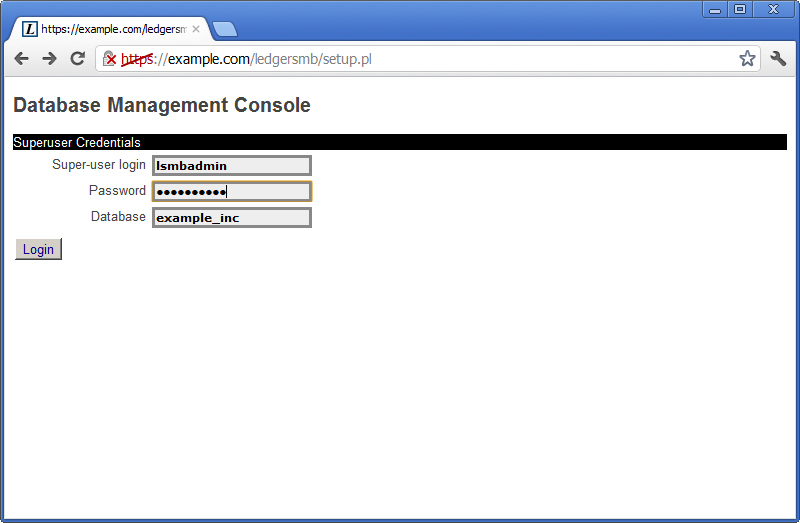
\includegraphics[width=0.8\textwidth]{dmc-create-step1.png}
		% HTML processing does not handle cropping of this image, need to figure out why?
		% 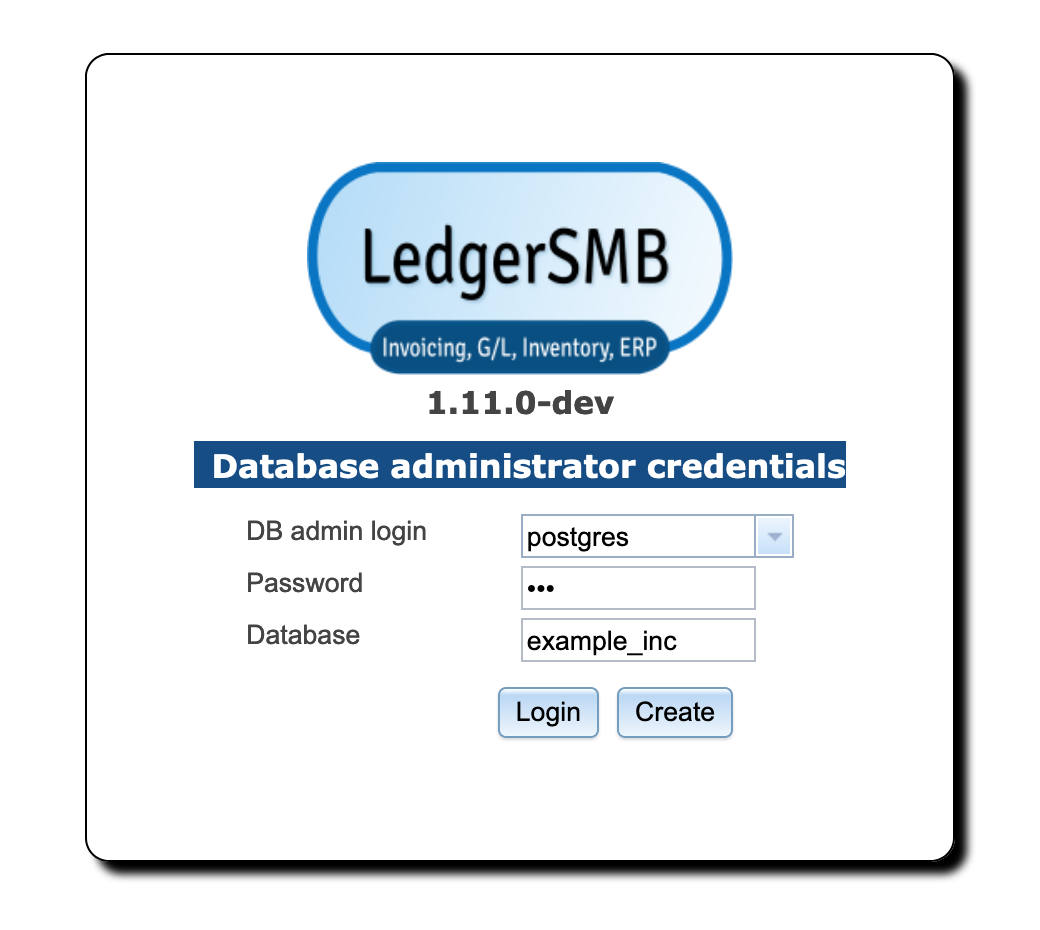
\includegraphics[width=\graphicswidth,  trim={0pt 50 0 0}, clip]{\autoscreenshotdir/setup-pl-login.png}
		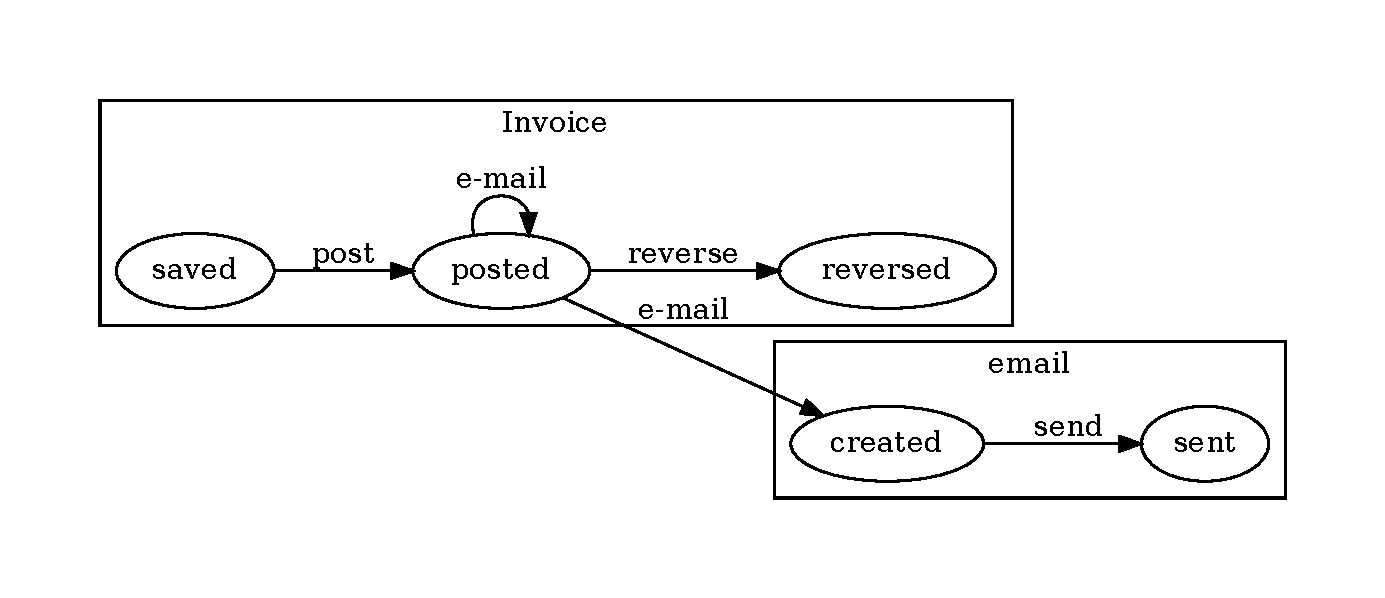
\includegraphics[width=\graphicswidth]{wf1.pdf}
		\caption{Workflow triggered from another workflow}
		\label{fig:triggered-workflow}
	\end{figure}
}{
	\begin{figure}
	\digraph[scale=0.4]{wf1}{
		rankdir=LR;
		subgraph invoice {
			graph [label="Invoice"];
			cluster = true;
			saved -> posted [label="post"];
			posted -> reversed [label="reverse"];
		};
	
	    subgraph email {
	    	graph [label="email"];
	    	cluster = true;
	    	created -> sent [label="send"];
	    };
	
	    posted -> created [label="e-mail"];
	    posted -> posted [label="e-mail"];
	
	}
	\caption{Workflow triggered from another workflow}
	\label{fig:triggered-workflow}
	\end{figure}
}

Actions belonging to a state may (or may not) be available. This is determined by one or
more conditions.  Examples are ``is the posting date of the transaction in a closed period''
and ``is the current user allowed to post transactions''.  When the condition evaluates to
\texttt{false}, the action is not available.

Workflows are configurable. Configurations list the following aspects:

\begin{enumerate}
	\item A list of states
	\item A list of allowable actions per state
	\item A list of conditions per action
	\item A mapping of actions to Perl code
	\item A mapping of conditions to Perl code
\end{enumerate}

With these ingredients, the software's behavior can be changed.  E.g. by adding a new state
and action in the invoice, an extra reviewing pairs of eyes can be added to the posting process.
By adding a condition on this action, it can be made required for invoices over 100.000 USD
(but not for other invoices).

\IfFileExists{./wf2.pdf}{
	\begin{figure}[H]
		\centering
		% 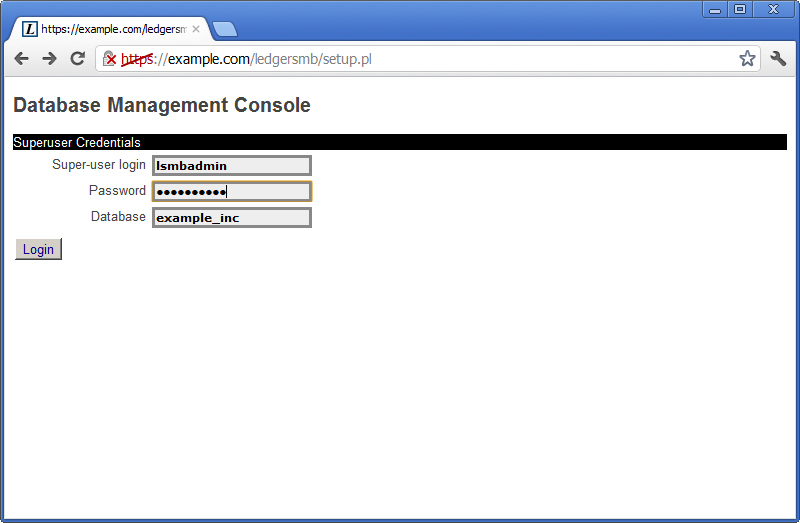
\includegraphics[width=0.8\textwidth]{dmc-create-step1.png}
		% HTML processing does not handle cropping of this image, need to figure out why?
		% 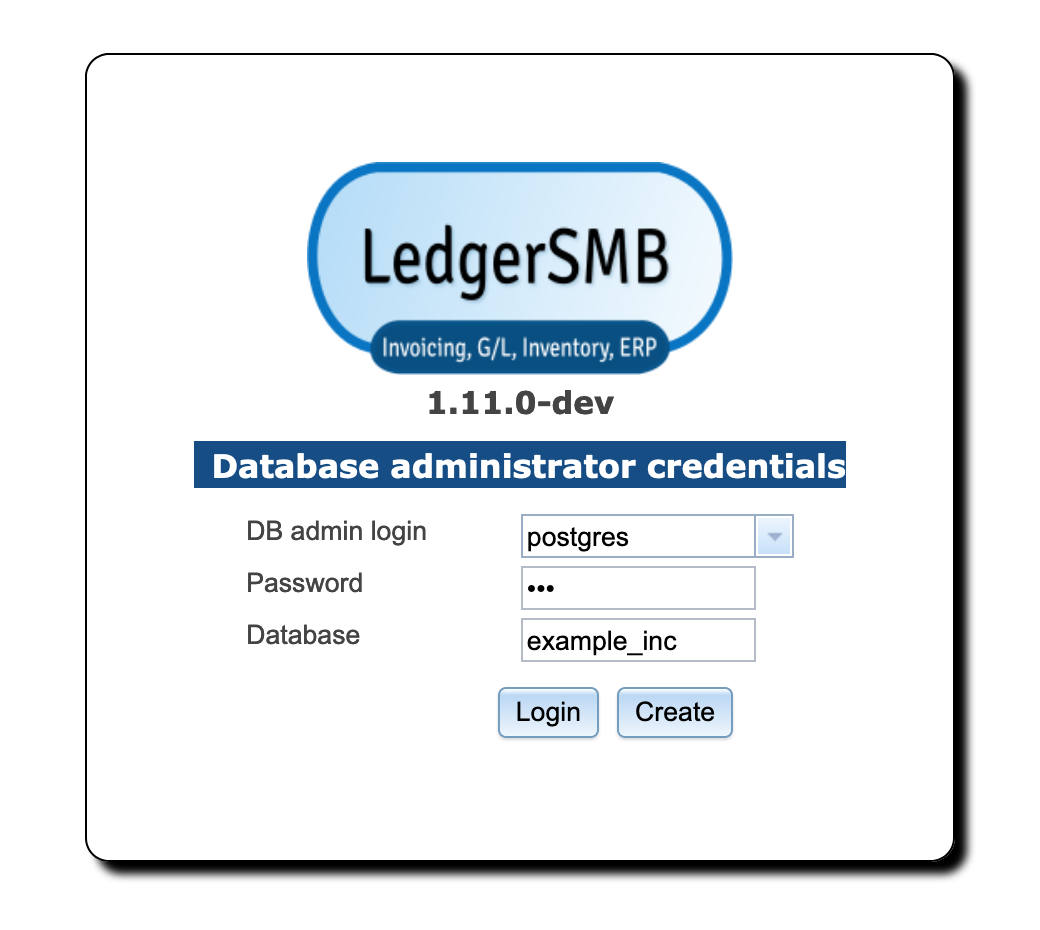
\includegraphics[width=\graphicswidth,  trim={0pt 50 0 0}, clip]{\autoscreenshotdir/setup-pl-login.png}
		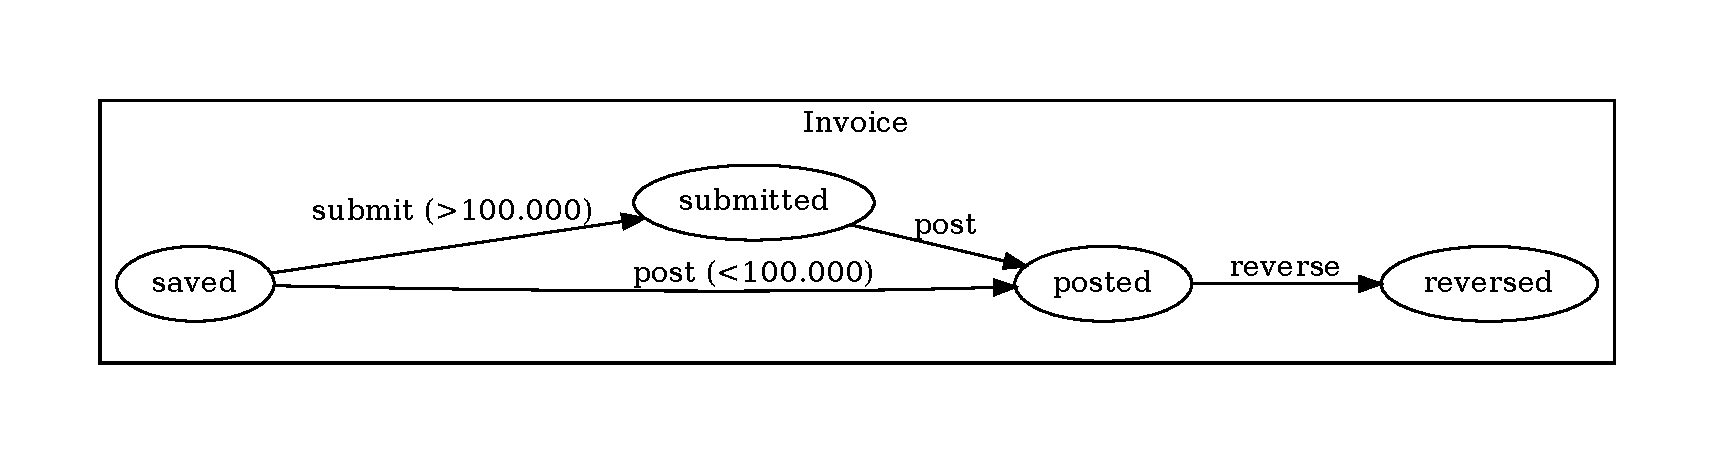
\includegraphics[width=\graphicswidth]{wf2.pdf}
		\caption{Conditional workflow actions}
		\label{fig:conditional-workflows}
	\end{figure}
}{
	\begin{figure}
		\digraph[scale=0.4]{wf2}{
			rankdir=LR;
			subgraph invoice {
				graph [label="Invoice"];
				cluster=true;
				saved -> posted [label="post (<100.000)"];
				saved -> submitted [label="submit (>100.000)"];
				submitted -> posted [label="post"];
				posted -> reversed [label="reverse"]
			}
		}
		\caption{Conditional workflow actions}
		\label{fig:conditional-workflows}
	\end{figure}
}

By changing association of the \texttt{save} action with its code, the application will act
differently when saving the invoice.  Customizations may associate new behaviors with existing
actions or create new ones entirely.  The behavior does not need to be known by the application
developers, as the association may point to code added to the local installation.  This way, a
\texttt{remind} action can be added to posted invoices, triggering a text (SMS) message to the
customer.


Workflows are stored in the \texttt{./workflows/} directory.  Each workflow consists of
several files, prefixed with the name of the workflow (e.g. \texttt{ar-ap.} for 'AR/AP' workflows):

\begin{description}
	\item [\texttt{ar-ap.actions.xml}] (optional) names the list of available transitions
	in the workflow naming Perl code to be executed
	\item [\texttt{ar-ap.conditions.xml}] (optional) names the list of conditions to be used
	in the workflow naming Perl code to evaluate
	\item [\texttt{ar-ap.persisters.xml}] (optional) defines the Perl mechanism to load and store
	workflow instances
	\item [\texttt{ar-ap.workflow.xml}] (required) defines the life cycle by combining states with
	the actions and conditions listed in the respective configuration files. Each state lists
	the allowable actions with the conditions to enable the action and a resulting state.
\end{description}

Customized versions of workflow definition files must be stored in \linebreak
 \texttt{./customized\_workflows/}\footnote{See
 	\secref{subsec-global-config-ledgersmb-yaml} on how to configure
 these paths}.  Files stored in this directory will be used to override those in
the standard location: the file\linebreak \texttt{./custom\_workflows/ar-ap.workflow.xml} will replace the built-in workflow
from \texttt{./workflows/ar-ap.workflow.xml} used for invoices and \linebreak AR/AP transactions.
No changes should be made directly to the standard files because of the risk that those
files will be overwritten on upgrade -- loosing the changes.

Next to the per-workflow files, there is a generic definition file for actions,
conditions and persisters.  Elements defined in these files can be used in all
workflows; those elements defined in the per-workflow files can only be used
in the specific workflow.

The engine driving workflow state management is the
Workflow\footnote{\url{https://metacpan.org/pod/Workflow}} library.  See its
documentation on MetaCPAN as well as the built-in workflows as examples of how
to define one's own.

\subsection{Workflow observers}
\label{subsec-customization-workflow-observers}

Particularly interesting is the concept of observers\index{workflow observers}:
this functionality allows the application to be extended based a specific action
occurring without changing the life cycle.  An example could be to create a PayPal
payment request when an invoice is posted: an observer could be ``listening'' to
``AR/AP'' workflow events which at some point will flag the state of the invoice
becoming \texttt{posted}.

\subsubsection{Notes on Quote, Order, AR, AP and GL workflow customization}
\label{subsubsec-customization-workflow-observers-notes}

The actions in the workflows \texttt{order-quote}, \texttt{ar-ap} and \texttt{gl} are
hard coded\footnote{This is not a permanent situation, but rather a consequence of
these workflows being used in \gls{oldcode}\index{old code}}.  This means that the list of actions is restricted to those defined in the
files \texttt{order-quote.actions.xml}, \texttt{ar-ap.actions.xml} and
\texttt{gl.actions.xml}.  It's not necessary to use all actions in the workflow, but
additional ones cannot be created -- contrary to what is in the \texttt{Workflow}
documentation.

The \texttt{class} attribute for most actions in these workflows is set to the value
\texttt{LedgerSMB::Workflow::Action::Null}.  This means it does nothing.  Rather, it
doesn't do anything \textit{in addition to} what the action already does in its hard
coded implementation.  Setting the action's class attribute to some other value allows
the developer to add behavior on top of what's hard coded.

\section{Document formatters}
\label{sec-customization-document-formatters}

Document formatters transform templates into output documents; e.g. an HTML invoice
template can be transformed into an HTML file with the details of the invoice filled
out.  LedgerSMB comes with a number of built-in formatters.  Additional ones could be
implemented to transform HTML documents to PDF (replacing the traditional \LaTeX to PDF)
or the creation of eInvoices\index{eInvoice} in the format of the local jurisdiction.

The generation of output entails these steps (preceded by the process to find a
suitable document formatter):

\begin{itemize}
	\item Loading the input template from the database
	\item Preprocessing the input variables using the formatter's \texttt{encode}
		function
	\item Initializing the template expansion using the formatter's \texttt{setup} function
	\item Expanding the template using \texttt{Template::Toolkit}
	\item Post-processing the expanded output using the formatter's \texttt{postprocess}
\end{itemize}

A custom formatter needs to implement the protocol as documented at \url{https://docs.ledgersmb.org/perl-api/1.11.0/LedgerSMB/Template.pm.html#FORMATS}.

\section{Bank statement importers}
\label{sec-customization-bank-importers}

LedgerSMB comes with three bank statement importers built-in:

\begin{itemize}
	\item [CAMT.053] The \gls{ISO20022}\index{ISO20022} ``Cash Management'' message 053
		(Bank-to-Customer account statement)
	\item [\gls{OFX}\index{OFX}] A standard to exchange data describing financial transactions
	\item [CSV]  File based using \gls{csv}\index{csv}
\end{itemize}

The bank statement importer is a Perl class implementing the
\texttt{LedgerSMB::Reconciliation::Format} role; it parses a file with bank
transactions, extracting the fields expected by the bank reconciliation procedure:

\begin{itemize}
	\item [amount] The amount involved in the transaction; negative if the bank
		reports a credit amount, positive when it's a debit
	\item [date] The date on which the amount contributed to the bank account balance
	\item [source] An identifier by which the bank identifies the transaction; to be
		used for matching with the ``Source'' field in the bank ledger
	\item [type] Information clarifying the transaction; e.g. Cash, ACH, etc.
\end{itemize}

The CSV parser has many options to accommodate the tremendous variance that can be
observed in CSV files.  When using a custom bank reconciliation procedure \textit{or}
when the bank makes a more exotic format available, customization of the bank statement
importer may be necessary.

\section{HTTP request interceptors}
\label{sec-customization-http-requests}

@@@TODO: describe how to add \texttt{Plack::Middleware} instances in the request processing

\section{Outgoing mail transport}
\label{sec-customization-outgoing-mail}

The library used for sending e-mail (\texttt{Email::Sender})
includes a wide variety of transports that can be used to configure the library to (pretend to) send
e-mail messages.  For a list of available transports, see \url{https://metacpan.org/dist/Email-Sender}.

Should a different delivery method be required even considering the list of available transports,
this can be achieved by implementing a custom \texttt{Email::Sender::Transport}.

\section{Sales/VAT tax calculation}
\label{sec-customization-sales-tax}

Tax calculations performed for VAT and/or sales taxes have been abstracted into so-called
``tax modules''.  An example of a custom tax module can be found in the directory
\texttt{utils/wa-tax-service} in the source repository.

Before tax modules can be used, they need to be registered in the \texttt{taxmodule} table.

\textbf{Important:} Please note that there is a tight integration between the database "pointing"
to the tax module and the web server which expects to be able to \textit{load} this Perl code to
perform the prescribed calculations.
If for some reason the application looses the ability to load the Perl module, this will break
the ability to create or view invoices.

\chapter{Batch data import methods}
\label{cha-customization-batch-import}

\section{Custom bank statement import}
\label{sec-customization-batch-import-bank-statement}

\section{Chart of Accounts import}
\label{subsec-customization-import-coa}

This function allows bulk import of an entire chart of accounts using a
single \gls{csv} file.

The first line of the file contains the headers of the columns. The
import routine expects the columns as presented in (table name).

\begin{description}
\item [accno] Number of the account or header
\item [desc] Description for the account or header
\item [charttype] ``H'' for heading record \\
``A'' for account record
\item [category] ``I'' for Income \\
``E'' for Expense \\
``A'' for Asset \\
``L'' for Liability
\item [contra] ``0'' not a \gls{contra}\index{contra} account \\
``1'' is a \gls{contra} account
\item [tax] ``0'' not a tax account \\
``1'' is a tax account.
\item [link] A colon (':') separated list of account check-mark values (links) as described
    in \secref{subsec-coa-account-links}, or ``AR'', ``AP'' or ``IC'' for the specified summary accounts
\item [heading] ``accno'' of the heading to group the account (or heading) under
\item [gifi] \gls{gifi} account number
\end{description}

All lines after the first one are considered to be data lines.

\chapter{Add-ons and plug-ins}
\label{cha-customization-add-ons}

\chapter{Company creation}
\label{cha-customization-company-creation}

\section{Template sets}\index{templates}
\label{sec-customization-company-creation-templates}
